\documentclass[12pt]{report}

% packages used for many things
\usepackage[utf8]{inputenc}
\usepackage[english]{babel}
\usepackage{hyperref}
\hypersetup{
    colorlinks=true,
    linkcolor=blue,
    filecolor=magenta,      
    urlcolor=cyan,
}
\urlstyle{same}
% package used for the enumeration
\usepackage{enumitem}
% packages used to write more symbols and text in math mode
\usepackage{amsmath}
\usepackage{mathtools}
\usepackage{amsfonts} 
\usepackage{amssymb}
\usepackage{MnSymbol}
\usepackage{csquotes}
\usepackage{arydshln}
\usepackage{algorithm}
\usepackage{algorithmic}

% for text over equal sign
\newcommand\prone{\mathrel{\overset{\makebox[0pt]{\mbox{\normalfont\tiny\sffamily (1)}}}{=}}}
\newcommand\prtwo{\mathrel{\overset{\makebox[0pt]{\mbox{\normalfont\tiny\sffamily (2)}}}{=}}}
\newcommand\prthr{\mathrel{\overset{\makebox[0pt]{\mbox{\normalfont\tiny\sffamily (3)}}}{=}}}


% for images
\usepackage{graphicx}
\graphicspath{{./images/}}

% qed black square
\newcommand*{\QEDA}{\hfill\ensuremath{\blacksquare}}


\title{Variational Autoencoder Mathematics}
\author{\LARGE{Andreas Spanopoulos} \\
        \LARGE{Demetrios Konstantinidis} \\ \\
        andrewspanopoulos@gmail.com \\
        demetris.konst@gmail.com}


% ----------------    START OF DOCUMENT    ------------ %
\begin{document}
\maketitle

% --------------------           PAGE 1           ---------------------- %
\section*{Introduction}
\smallskip

The \textbf{Variational Autoencoder} (aka \textbf{VAE}) is a generative model.
This means that it is a model which produces new unseen data. Unlike the normal
Autoencoder, VAE focuses on understanding the distribution of a smaller
representation of the data. This lower-dimensional representation of the data is
known as \textquote{latent vector $\textbf{z}$}.
\bigskip

The dimension of the latent vector z is a hyperparameter which we choose along
with the architecture of the Network. Keep in mind that we don't want
$\textbf{z}$ to be too large. It should be a relatively small vector, so that an
information bottleneck is created. One other reason for $\textbf{z}$ being small,
is that we want to be able to sample easily new vectors, without having to take
into consideration many features.
\bigskip

With that said, the question arises: How can we pick the values of $\textbf{z}$
which will make sense, that is, which will generate a new data point from the
distribution of our original data?
\bigskip

Here is the beauty of the \textbf{Variational Autoencoder}: We will learn the
distribution of $\textbf{z}$. That is, for every component of $\textbf{z}$, we
will learn a mean and a standard deviation.
\bigskip

Suppose $\textbf{z}$ has $k$ components:
\begin{align*}
    z \;=\;
    \begin{bmatrix}
        z_1 \\
        z_2 \\
        \vdots \\
        z_k
    \end{bmatrix}
\end{align*}
Then, the mean and standard deviation vectors are defined as:
\begin{align*}
    \mu \;=\;
    \begin{bmatrix}
        \mu_1 \\
        \mu_2 \\
        \vdots \\
        \mu_k
    \end{bmatrix}
    ,\quad \sigma \;=\;
    \begin{bmatrix}
        \sigma_1 \\
        \sigma_2 \\
        \vdots \\
        \sigma_k
    \end{bmatrix}
\end{align*}
Our goal is to learn the $\mu$ and $\sigma$ vectors in order to be able to sample
$\textbf{z}$ as follows $$z \;=\; \mu + \epsilon \odot \sigma$$
where $\epsilon \sim N(0, 1)$ is a gaussian with mean 0 and standard deviation 1.
\clearpage

% --------------------           PAGE 2           ---------------------- %
\begin{figure}
    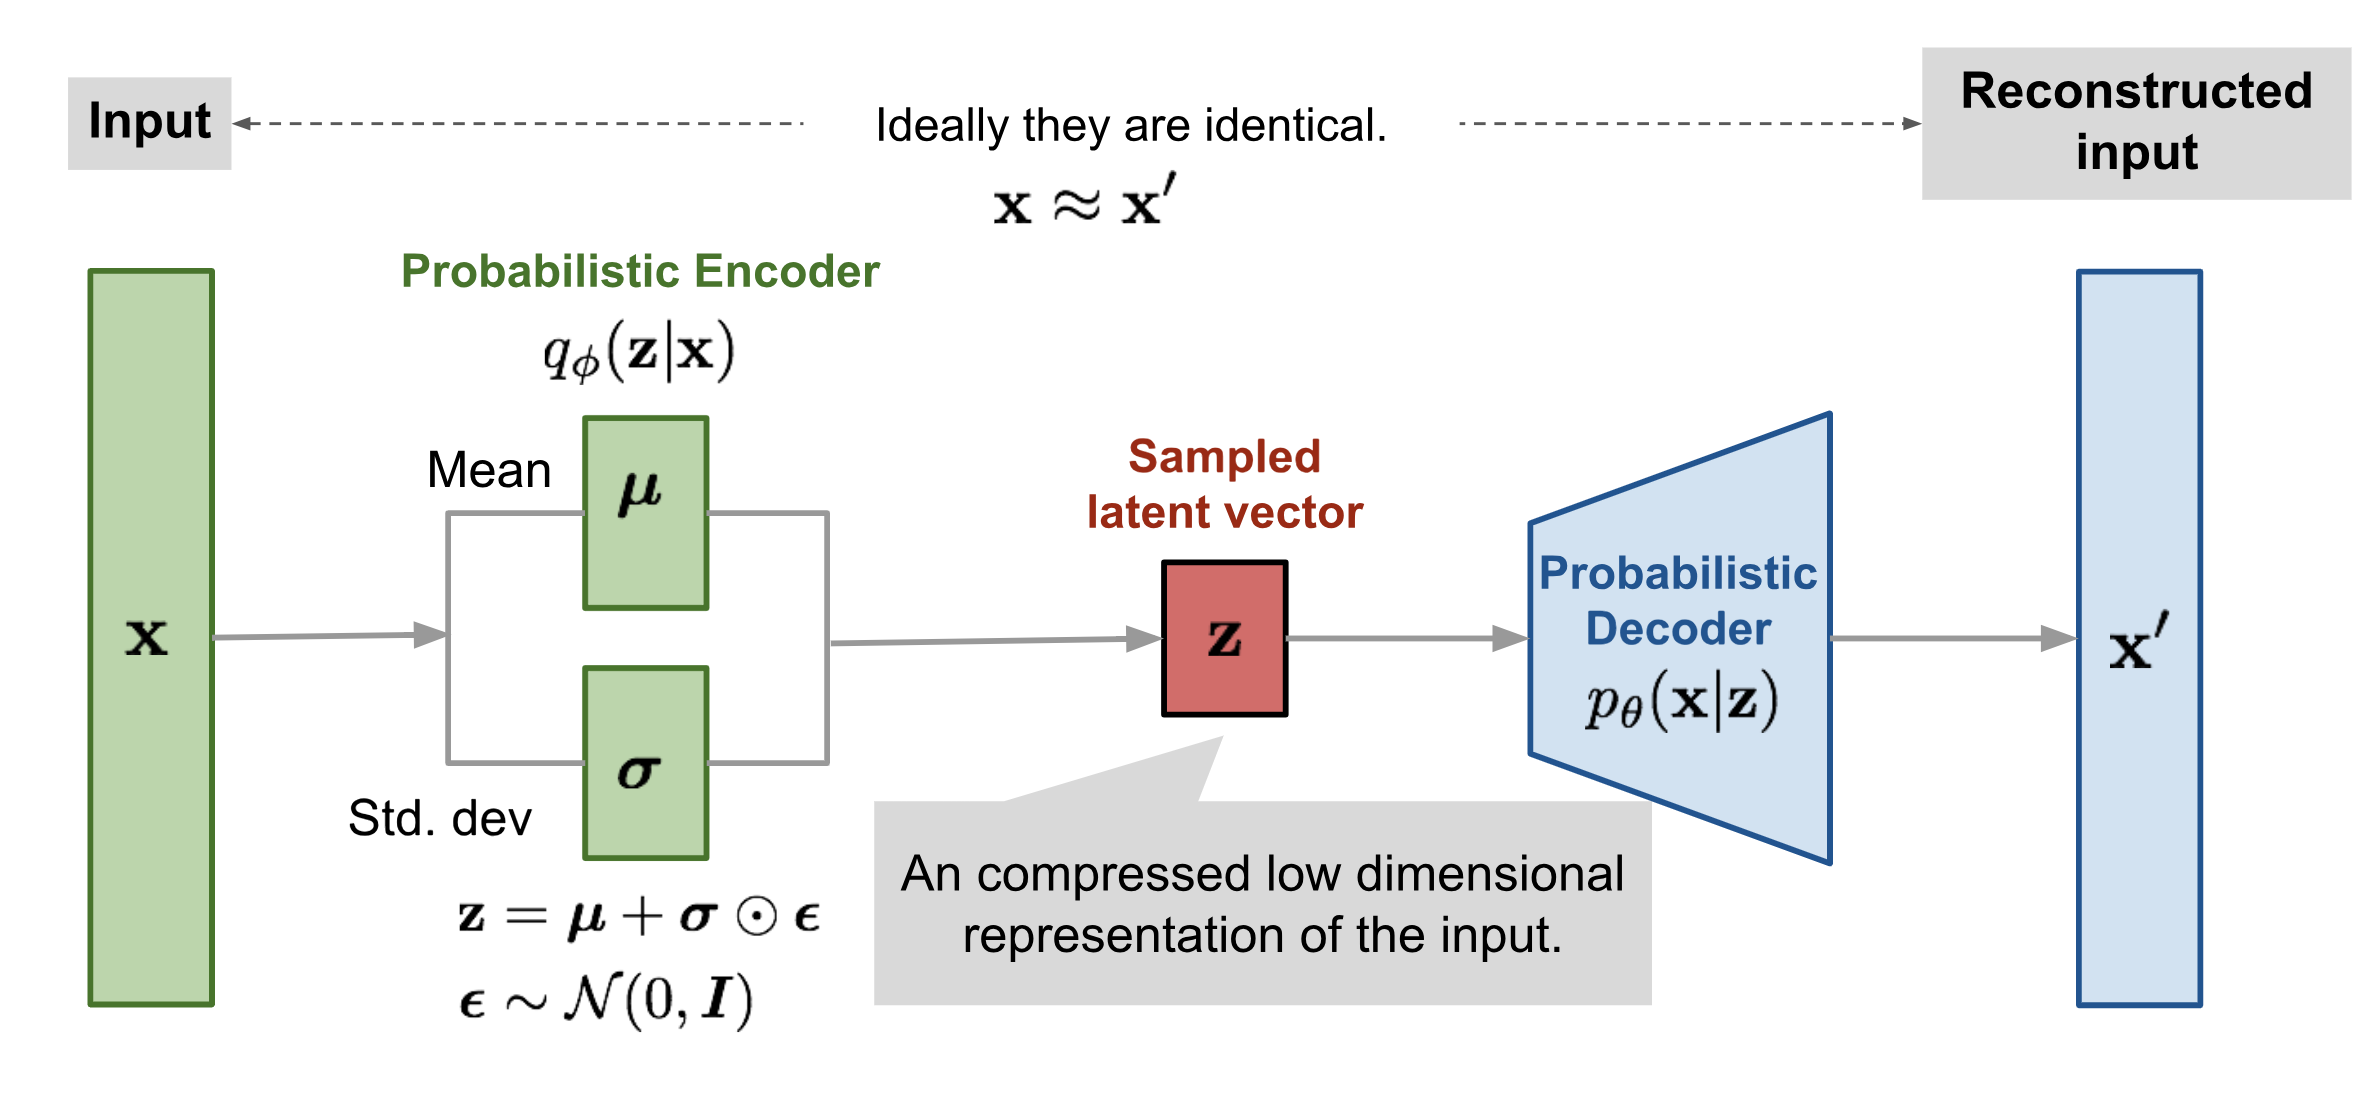
\includegraphics[scale=0.31]{vae-gaussian.png}   
    \caption{This picture demonstrates the architecture of a Variational
             Autoencoder. The input \textbf{x} gets fed in a Probabilistic
             Encoder $q_{\phi}(z | x)$, which in turns connects with the
             $\mu$ and $\sigma$ layers. Note that usually there is a encoder
             Network before the mean and std layers, but here in the figure
             it is ommitted. Then, they sample $\textbf{z}$ which
             in turn is fed to the Probabilistic Decoder $p_{\theta}(x | z)$.
             The result is then fed to an output layer which represents the
             reconstructed input data. The original picture can be found
             \href{https://blog.bayeslabs.co/2019/06/04/All-you-need-to-
             know-about-Vae.html}{here}.}
    \label{fig:Architecture}
\end{figure}

\subsection*{Brief Explanation of architecture}
The architecture of a \textbf{VAE} is briefly portrayed in 
Figure~\ref{fig:Architecture}. Let's take a closer look in each part:

\begin{enumerate}
    \item The encoder part consists of a Probabilistic Encoder $q_{\phi}(z | x)$.
        Given some parameters $\phi$ (which are parameters of the model),
        $q_{\phi}(z | x)$ models the probability of obtaining the latent vector
        $\textbf{z}$ given input data $\textbf{x}$. Afterwards, it connects to
        the $\mu$ and $\sigma$ layers, as there might a whole encoder network
        before those.
    \item The latent vector $\textbf{z}$.
    \item The decoder part which consists of a Probabilistic Decoder
        $p_{\theta}(x | z)$. As with the probabilistic encoder, given some
        parameters $\theta$ which are parameters of the model, we want to learn
        the probability of obtaining a data point $\textbf{x}$ given a latent
        vector $\textbf{z}$.
    \item The reconstructed input $\hat{x}$.
\end{enumerate}
\clearpage

% --------------------           PAGE 3           ---------------------- %
\section*{Loss function}
The loss function of the VAE is:
\begin{align*}
    L(\theta,\, \phi,\, x) \;=\; -E_{z \sim Q_{\phi}(z | x)}
                                    \left[\log(P(x | z)) \right]\;
                              +\; D_{KL}\left[Q_{\phi}(z | x) \;||\; P(z) \right]
\end{align*}
It may seem daunting at first, but if we break it down into pieces then it gets
much simpler.

\subsection*{KL-Divergence and multivariate Normal Distribution}
Let's start by explaining what the second term of the loss function is. The
\textbf{K}ullback \textbf{L}eiber Divergence, also known as
\href{https://en.wikipedia.org/wiki/Relative_entropy}{Relative Entropy}, is
a measure of similarity between two probability distributions. It is denoted by
$D_{KL}(\cdot \;||\; \cdot)$, its unit of measure it called \textbf{nat} and it
can computed by the formula (for discrete probability distributions):
\begin{equation}\label{eq:KLD}
    D_{KL} (P \,||\, Q) \;=\; \sum_x P(x) \log\left(\frac{P(x)}{Q(x)}\right)
\end{equation}
Of course, this implies that $D_{KL} (P \,||\, Q) \neq D_{KL} (Q \,||\, P)$.
\bigskip

Now, let's suppose that both $P,\; Q$ are multivariate
normal distributions with means $\mu_1, \mu_2$ and
\href{https://en.wikipedia.org/wiki/Covariance_matrix}{covariance} matrices
$\Sigma_1, \Sigma_2$:
\begin{align*}
P(x) \,=&\, N(x;\, \mu_1,\, \Sigma_1) \,=\,
    \frac{1}{\sqrt{(2\pi)^k|\Sigma_1|}}
    e^{-\frac{1}{2}(x-\mu_1)^T\Sigma_1^{-1}(x - \mu_1)} \\
Q(x) \,=&\, N(x;\, \mu_2,\, \Sigma_2) \,=\,
    \frac{1}{\sqrt{(2\pi)^k|\Sigma_2|}}
    e^{-\frac{1}{2}(x-\mu_2)^T\Sigma_2^{-1}(x - \mu_2)}
\end{align*}
where $k$ is the magnitude (length) of vector $x$.
\smallskip

\noindent Hence
\begin{align*}
    \log(P(x)) \;=\;& \log\left(\frac{1}{\sqrt{(2\pi)^k|\Sigma_1|}}
                e^{-\frac{1}{2}(x-\mu_1)^T\Sigma_1^{-1}(x - \mu_1)} \right) \\
               \;=\;& \log \left( \frac{1}{\sqrt{(2\pi)^k|\Sigma_1|}} \right) +
                \log \left( e^{-\frac{1}{2}(x-\mu_1)^T\Sigma_1^{-1}
                (x - \mu_1)} \right) \\
               \;=\;& -\frac{k}{2}\log(2\pi) -\frac{1}{2}\log(|\Sigma_1|) -
                \frac{1}{2}(x-\mu_1)^T\Sigma_1^{-1} (x - \mu_1)
\end{align*}
\clearpage

% --------------------           PAGE 4           ---------------------- %
\noindent Following the exact same steps, we also get that
\begin{align*}
    \log(Q(x)) \;=\; -\frac{k}{2}\log(2\pi) -\frac{1}{2}\log(|\Sigma_2|) -
    \frac{1}{2}(x-\mu_2)^T\Sigma_2^{-1} (x - \mu_2)
\end{align*}

\noindent With the help of the above equalities, expanding \eqref{eq:KLD} yields:

\begin{align*}
    D_{KL} (P \,||\, Q)
    \;=&\; \sum_x P(x) \left[\log(P(x)) - \log(Q(x)) \right] \\
    \;=&\; \sum_x P(x) \left[ \frac{1}{2}\log\left(\frac{|\Sigma_2|}{|\Sigma_1|}\right)
        - \frac{1}{2}(x-\mu_1)^T\Sigma_1^{-1} (x - \mu_1) \right. \\
       &\left.\qquad\qquad\qquad\qquad\quad\;\;\;\,
        + \frac{1}{2}(x-\mu_2)^T\Sigma_2^{-1} (x - \mu_2)\right]
\end{align*}
We can rewrite the above term an an Expectation over $P$:
\begin{align*}
    D_{KL} (P \,||\, Q)
    \;=&\; E_P \left[ \frac{1}{2}\log\left(\frac{|\Sigma_2|}{|\Sigma_1|}\right)
        - \frac{1}{2}(x-\mu_1)^T\Sigma_1^{-1} (x - \mu_1) \right. \\
       &\left.\qquad\qquad\qquad\quad\;\;\,
        + \frac{1}{2}(x-\mu_2)^T\Sigma_2^{-1} (x - \mu_2)\right]
\end{align*}
Since the logarithmic term is independent of $x$, we can move it outside the
expectation. This leaves us with
\begin{align}\label{eq:kld_exp}
    D_{KL} (P \,||\, Q)
    \;=\quad &\frac{1}{2}\log\left(\frac{|\Sigma_2|}{|\Sigma_1|}\right) \nonumber \\
       \; -\, &\frac{1}{2} E_P \left[ (x-\mu_1)^T\Sigma_1^{-1} (x - \mu_1) \right]
            \nonumber \\
       \; +\, &\frac{1}{2} E_P \left[ (x-\mu_2)^T\Sigma_2^{-1} (x - \mu_2) \right]
\end{align}
Let's now try to simplify the 2nd and 3rd terms of the above expression.
\bigskip

\noindent First, we have to recall the
\href{https://en.wikipedia.org/wiki/Trace_(linear_algebra)}{trace}
function and some of its properties. The trace of a square matrix $A$,
denoted as $tr(A)$, is the sum of the elements along the main diagonal of $A$.
The \href{https://en.wikipedia.org/wiki/Trace_(linear_algebra)#Properties}{properties}
of the trace function which we will need are:
\begin{enumerate}
    \item \href{https://math.stackexchange.com/questions/3098841/how-could-a-scalar-
        be-equal-to-the-trace-of-the-same-scalar}{Trace of scalar}:
        Considering the scalar as a $1\times1$ matrix, gives: $x = tr(x)$
    \item \href{https://math.stackexchange.com/questions/2228398/trace-trick-for-
        expectations-of-quadratic-forms}{Trace of Expectation}:
        From 1: $E[x] = E[tr(x)] \Rightarrow tr(E[x]) = E[tr(x)]$
    \item \href{https://en.wikipedia.org/wiki/Trace_(linear_algebra)#Cyclic_property}
        {Cyclic Property}: $tr(ABC) \;=\; tr(CAB)$
\end{enumerate}
\clearpage

% --------------------           PAGE 5            ---------------------- %
\noindent Having these properties in mind, we are now ready to simplify the
expectation terms computed before during the simplification of the KL Divergence.

\begin{itemize}
    \item Term 2. Note that the matrix multiplications inside the expectation reduces
        to a scalar value.
        \begin{align*}
            E_P \left[ (x-\mu_1)^T\Sigma_1^{-1} (x - \mu_1) \right]
            \;\prone\;& E_P \left[ tr\left((x-\mu_1)^T\Sigma_1^{-1}
                (x - \mu_1)\right) \right] \\
            \;\prthr\;& E_P \left[ tr\left( (x - \mu_1)(x - \mu_1)^T
                \Sigma_1^{-1} \right) \right] \\
            \;\prtwo\;& tr\left( E_P\left[ (x - \mu_1)(x - \mu_1)^T
                \Sigma_1^{-1} \right] \right)
        \end{align*}
        $\Sigma_1^{-1}$ is independent from the expectation over $P$, so it can be moved
        outside, giving:
        \begin{align*}
            E_P \left[ (x-\mu_1)^T\Sigma_1^{-1} (x - \mu_1) \right] \;=\;
                tr\left( E_P\left[ (x - \mu_1)(x - \mu_1)^T
                    \right] \Sigma_1^{-1} \right)
        \end{align*}
        But the term $E_P\left[ (x - \mu_1)(x - \mu_1)^T \right]$ is equal to the
        \href{https://en.wikipedia.org/wiki/Covariance_matrix#Definition}
        {Covariance Matrix} $\Sigma_1$, thus yielding
        \begin{align}\label{eq:kld_term2}
            E_P \left[ (x-\mu_1)^T\Sigma_1^{-1} (x - \mu_1) \right]
                \;=\; tr\left( \Sigma_1 \Sigma_1^{-1} \right) \;=\; tr(I_k) \;=\; k
        \end{align}
    \item Term 3. Again, the term inside the expectation reduces to a scalar.
        \begin{align*}
            E_P &\left[ (x - \mu_2)^T\Sigma_2^{-1} (x - \mu_2) \right] \\[1ex]
            \mbox{Add and}& \mbox{ subtract } \mu_1: \\[1ex]
            \;=&\; E_P \left[ [(x - \mu_1) + (\mu_1 - \mu_2)]^T\Sigma_2^{-1}
                [(x - \mu_1) + (\mu_1 - \mu_2)] \right] \\[2ex]
            \;=&\; E_P \left[ \left[(x - \mu_1)^T + (\mu_1 - \mu_2)^T\right]
                \Sigma_2^{-1} [(x - \mu_1) + (\mu_1 - \mu_2)] \right] \\[2ex]
            (A^T + B^T&)C(A + B) \;=\; A^TCA + A^TCB + B^TCA + B^TB: \\[2ex]
            \;=&\; E_P \left[ (x - \mu_1)^T\Sigma_2^{-1}(x - \mu_1) \;+\;
                (x - \mu_1)^T\Sigma_2^{-1}(\mu_1 - \mu_2) \;+ \right. \\[2ex]
                & \quad\;\;\;\,
                \left. (\mu_1 - \mu_2)^T\Sigma_2^{-1}(x - \mu_1) \;+\; 
                (\mu_1 - \mu_2)^T\Sigma_2^{-1}(\mu_1 - \mu_2) \right] \\[2ex]
            A^TCB \;=&\; B^TCA: \\[2ex]
            \;=&\; E_P \left[ (x - \mu_1)^T\Sigma_2^{-1}(x - \mu_1) \;+\;
                2(x - \mu_1)^T\Sigma_2^{-1}(\mu_1 - \mu_2) \;+ \right. \\[2ex]
                & \quad\;\;\;\,
                \left. (\mu_1 - \mu_2)^T\Sigma_2^{-1}(\mu_1 - \mu_2) \right]
        \end{align*}
        \clearpage
% --------------------           PAGE 6            ---------------------- %
        Taking the expectation over each term individually:
        \begin{align*}
            E_P \left[ (x - \mu_2)^T\Sigma_2^{-1} (x - \mu_2) \right]
            \;=\; &E_P \left[ (x - \mu_1)^T\Sigma_2^{-1}(x - \mu_1) \right] \;+\\[2ex]
                  &E_P \left[ 2(x - \mu_1)^T\Sigma_2^{-1}(\mu_1 - \mu_2) \right.]\;+\\[2ex]
                  &E_P \left[ (\mu_1 - \mu_2)^T\Sigma_2^{-1}(\mu_1 - \mu_2) \right]
        \end{align*}
        \begin{itemize}
            \item The first sub-term has the same derivation as the first term from before:
                $$E_P \left[ (x - \mu_1)^T\Sigma_2^{-1}(x - \mu_1) \right] \;=\;
                    tr(\Sigma_1\Sigma_2^{-1})$$
            \item The second sub-term is equal to $0$ due to the expectation over
                $(x - \mu_1)^T$. Specifically, the factor $\Sigma_2^{-1}(\mu_1 - \mu_2)$
                can be moved out of the expectation as it is a constant:
                \begin{align*}
                    E_P \left[ 2(x - \mu_1)^T\Sigma_2^{-1}(\mu_1 - \mu_2) \right.]
                    \;=&\; 2E_P \left[ (x - \mu_1)^T \right]
                        \Sigma_2^{-1}(\mu_1 - \mu_2) \\
                    \;=&\; 0_k \; \Sigma_2^{-1}(\mu_1 - \mu_2) \\
                    \;=&\; 0
                \end{align*}
            \item The third sub-term is the expectation of a constant, so it is equal
                to the constant itself:
                $$E_P \left[ (\mu_1 - \mu_2)^T\Sigma_2^{-1}(\mu_1 - \mu_2)\right] \;=\;
                (\mu_1 - \mu_2)^T\Sigma_2^{-1}(\mu_1 - \mu_2)$$
        \end{itemize}
    These simplifications leave us with:
    \begin{align}\label{eq:kld_term3}
        E_P \left[ (x - \mu_2)^T\Sigma_2^{-1} (x - \mu_2) \right] \;=\;\,
        &tr(\Sigma_1\Sigma_2^{-1}) \,+ \nonumber \\
        &(\mu_1 - \mu_2)^T\Sigma_2^{-1}(\mu_1 - \mu_2)
    \end{align}
\end{itemize}

\noindent Finally, formula \eqref{eq:kld_exp} for the KL-Divergence can be ultimately
simplified using equations \eqref{eq:kld_term2}, \eqref{eq:kld_term3} to:
\begin{align}
    D_{KL} (P \,||\, Q) \;=\;
    \frac{1}{2}\log\left(\frac{|\Sigma_2|}{|\Sigma_1|}\right) \;+\;
    k \;+\;
    tr(\Sigma_1\Sigma_2^{-1}) \;+\; (\mu_1 - \mu_2)^T\Sigma_2^{-1}(\mu_1 - \mu_2)
\end{align}
\QEDA

\end{document}
% ----------------    END OF DOCUMENT    ------------ %
